
\section{Vektorgeometrie}
\subsection{Grunddefinitionen}
\textbf{Vektor:}

Ein Vektor ist festgelegt durch eine Laenge (Groesse) und eine Richtung.

\textbf{Freie Vektoren: }
Sie beschreiben Merkmale,
bei denen es nur auf Groesse und Richtung ankommt

\textbf{Ortsvektoren:}
Sie beschreiben Merkmale,
bei denen es auf Groesse, Richtung und Anfangspunkt ankommt

Unter einem Ortsvektor $\vec{v}$  versteht man eine Strecke, bei der der eine der beiden Begrenzungspunkte als Anfangspunkt P, der andere Endpunkt Q festgelegt ist. Man schreibt $\vec{v} = \vec{PQ}$

\subsection{Grundrechenarten}
\subsubsection{Addition von Vektoren}
\includegraphics[scale=0.7]{vec1.PNG}
\subsubsection{Multiplikation mit einer Zahl}
\includegraphics[scale=0.7]{vec3.PNG}

\includegraphics[scale=0.7]{vec3-1.PNG}

\includegraphics[scale=0.7]{vec3-2.PNG}

\subsubsection{Skalarprodukt}
\includegraphics[scale=0.7]{vec4.PNG}

\includegraphics[scale=0.7]{vec4-1.PNG}

\includegraphics[scale=0.7]{vec4-2.PNG}

\subsubsection{Vektorprodukt}
\includegraphics[scale=0.7]{vec5.PNG}
\newpage{}
\begin{multicols*}{2}
    \subsubsection{Betrag eines Vektors}
    Die Laenge eines Vektors heisst Betrag des Vektors.
    \[\vec{v}= \begin{pmatrix} x \\ y \end{pmatrix} \Longrightarrow \left|\vec{v}\right| = \sqrt{x^2 + y^2}\]
    \subsubsection{Einheitsvektor}
    Ein Vektor der Laenge heisst Einheitsvektor. \\
    Die Formel für die Berechnung des Einheitsvektors $\vec{a}^0$ lautet:
    \[\vec{a}^0 = \frac{1}{|a|} \vec{a}\]

    \subsection{Normalform}
    \subsubsection{Normalform einer Gerade}
    Eine Gerade laesst sich lediglich im $\mathbb{R}^2$ in Normalenform darstellen, weil es im $\mathbb{R}^3$ keinen eindeutigen Normalenvektor gibt.
    \[g\colon\; \vec{n} \circ [\vec{x} - \vec{a}] = 0\]

    \begin{itemize}
        \item  $\vec{g}$: Bezeichnung der Gerade
        \item  $\vec{n}$: Normalenvektor (Vektor, der senkrecht auf der Gerade steht)
        \item  $\vec{a}$: Aufpunkt (oder: Stuetzvektor)
    \end{itemize}
    \subsubsection{Normalform einer Ebene}
    \[E\colon\; \vec{n} \circ [\vec{x} - \vec{a}] = 0\]

    \begin{itemize}
        \item  $\vec{E}$: Bezeichnung der Ebene
        \item  $\vec{n}$: Normalenvektor (Vektor, der senkrecht auf der Gerade steht)
        \item  $\vec{a}$: Aufpunkt (oder: Stuetzvektor)
    \end{itemize}
    \subsubsection{Hessesche Normalform einer Gerade}
    \[g\colon\; \vec{n}_0 \circ [\vec{x} - \vec{a}] = 0\]
    \begin{itemize}
        \item  $\vec{n}$: Normalenvektor (Vektor, der auf einer Gerade senkrecht steht)
        \item  $\vec{n}_0$: Normierter Normalenvektor (Normalenvektor der Länge 1) $\vec{n}_0 = \frac{\vec{n}}{|\vec{n}|}$
        \item  $|\vec{n}|$: Laenge des Normalenvektors
        \item  $\vec{a}$: Aufpunkt (oder: Stuetzvektor)
    \end{itemize}

    Gegeben sei die Gerade g in Normalenform mit

    \[g\colon\; \vec{n} \circ \left[\vec{x} - \vec{a}\right] = \begin{pmatrix} 4 \\ 3 \end{pmatrix} \circ \left[\begin{pmatrix} x_1 \\ x_2 \end{pmatrix} - \begin{pmatrix} 2 \\ 1 \end{pmatrix}\right] = 0\]
    Länge des Normalenvektors berechnen:
    \[ |\vec{n}| = \sqrt{4^2 + 3^2} = \sqrt{25} = 5\]
    Gerade in Hessescher Normalform aufstellen
    \[g\colon\; \frac{\vec{n}}{|\vec{n}|} \circ \left[\vec{x} - \vec{a}\right] = \frac{1}{5} \cdot \begin{pmatrix} 4 \\ 3 \end{pmatrix} \circ \left[\begin{pmatrix} x_1 \\ x_2 \end{pmatrix} - \begin{pmatrix} 2 \\ 1 \end{pmatrix}\right] = 0\]

    Oder Gegeben sei die Gerade n in Koordinatenform mit:
    \[g\colon\; 4x_1 - 3x_2 - 5 = 0\]
    Normalenvektor aus Koordinatenform herauslesen

    Die Koordinaten des Normalenvektors entsprechen den Koeffizienten von $x_1$ und $x_2$ in der Koordinatenform.
    \[\vec{n} = \begin{pmatrix} 4 \\ -3 \end{pmatrix}\]
    Laenge des Normalenvektors berechnen
    \[|\vec{n}| = \sqrt{4^2 + (-3)^2} = \sqrt{25} = 5\]
    Gerade in Hessescher Normalform aufstellen
    \[g\colon\; \frac{1}{5} \cdot [4x_1 - 3x_2 - 5] = 0\]

    \subsubsection{Hessesche Normalform einer Ebene}
    \[E\colon\; \vec{n}_0 \circ [\vec{x} - \vec{a}] = 0\]
    \begin{itemize}
        \item  $\vec{n}$: Normalenvektor (Vektor, der auf einer Ebene senkrecht steht)
        \item  $\vec{n}_0$: Normierter Normalenvektor (Normalenvektor der Länge 1) $\vec{n}_0 = \frac{\vec{n}}{|\vec{n}|}$
        \item  $|\vec{n}|$: Laenge des Normalenvektors
        \item  $\vec{a}$: Aufpunkt (oder: Stuetzvektor)
    \end{itemize}
    Gegeben sei die Ebene E in Normalenform mit
    \[E\colon\; \vec{n} \circ \left[\vec{x} - \vec{a}\right] = \begin{pmatrix} 2 \\ 1 \\ -2 \end{pmatrix} \circ \left[\begin{pmatrix} x_1 \\ x_2 \\ x_3 \end{pmatrix} - \begin{pmatrix} 0 \\ 1 \\ 1 \end{pmatrix}\right] = 0\]
    Laenge des Normalenvektors berechnen
    \[|\vec{n}| = \sqrt{2^2 + 1^2 + (-2)^2} = \sqrt{9} = 3\]
    Ebene in Hessescher Normalform aufstellen
    \[E\colon\; \frac{\vec{n}}{|\vec{n}|} \circ \left[\vec{x} - \vec{a}\right] = \frac{1}{3} \cdot \begin{pmatrix} 2 \\ 1 \\ -2 \end{pmatrix} \circ \left[\begin{pmatrix} x_1 \\ x_2 \\ x_3 \end{pmatrix} - \begin{pmatrix} 0 \\ 1 \\ 1 \end{pmatrix}\right] = 0\]

\end{multicols*}

\newpage{}

\subsection{Rechnen mit Vektoren}
\subsubsection{Dreiecksgleichung}
\begin{tikzpicture}[thick]
    \coordinate [label=below left:$A$] (A) at (0cm,0cm);
    \coordinate [label=above:$B$] (B) at (3cm,3cm);
    \coordinate [label=above:$C$](C) at (7cm,3cm);
    \coordinate (D) at (-6cm,0cm);
    \coordinate (E) at (-3cm,3cm);
    \coordinate (F) at (-5cm,4cm);
    \coordinate (G) at (-1cm,4cm);

    \draw [blue, -Latex, very thick] (A) -- node[above left,black] {\large $\vv{a}$} (B);
    \draw [blue, -Latex, very thick] (B) -- node[above,black] {\large $\vv{b}$} (C);
    \draw [red, -Latex, very thick] (A) -- node[below right,black] {\large $\vv{c} =\vv{a}+\vv{b}$} (C);
    \draw [blue, -Latex, very thick] (D) -- node[above left,black] {\large $\vv{a}$} (E);
    \draw [blue, -Latex, very thick] (F) -- node[above,black] {\large $\vv{b}$} (G);

    \draw [fill=black] (A) circle (1.5pt);% node [above] {A};
    \draw [fill=black] (B) circle (1.5pt);% node [right] {B};
    \draw [fill=black] (C) circle (1.5pt);
\end{tikzpicture}

\subsubsection{Addition von Vektoren}
Es seien $\vv{a} = \vv{AB}$ und  $\vv{b} = \vv{AD}$ zwei Vektoren.
Dann setzt man $\vv{a} +\vv{b} =  \vv{AC}$ wobei C der 4. Eckpunkt des Parallelograms ist.

\begin{tikzpicture}[thick]
    \coordinate [label=below left:$A$](A) at (0cm,0cm);
    \coordinate [label=above:$B$](B) at (3cm,3cm);
    \coordinate [label=above:$C$](C) at (7cm,3cm);
    \coordinate (D) at (-6cm,0cm);
    \coordinate (E) at (-3cm,3cm);
    \coordinate (F) at (-5cm,4cm);
    \coordinate (G) at (-1cm,4cm);
    \coordinate [label=below:$D$] (H) at (4cm,0cm);


    \draw [blue, -Latex, very thick] (A) -- node[above left,black] {\large $\vv{a}$}(B);
    \draw [dashed] (B) -- (C);
    \draw [red, -Latex, very thick] (A) -- (C);
    \draw [blue, -Latex, very thick] (A) -- node[below,black] {\large $\vv{b}$}(H);
    \draw [dashed] (H) -- (C);
    \draw [blue, -Latex, very thick] (D) -- node[above left,black] {\large $\vv{a}$}(E);
    \draw [blue, -Latex, very thick] (F) -- node[above,black] {\large $\vv{b}$}(G);

    \draw [fill=black] (A) circle (1.5pt);% node [above] {A};

    \draw (8.3cm,2.6cm) node {\large $\vv{c} =\vv{a}+\vv{b}$};

\end{tikzpicture}

Kommunativgestez:  $\vv{a}+\vv{b} =\vv{b}+\vv{a}$ \\
Assoziativgesetz: $(\vv{a}+\vv{b})+\vv{c} =\vv{a}+(\vv{b}+\vv{c})$



\subsubsection{Vektor Subtrahieren}
\begin{tikzpicture}[thick]
    \coordinate [label=below:$O$](A) at (2cm,0cm);
    \coordinate [label=above:$A$](B) at (5cm,3cm);
    \coordinate [label=above:$B$](C) at (1cm,3cm);
    \coordinate (D) at (-6cm,0cm);
    \coordinate (E) at (-3cm,3cm);
    \coordinate (F) at (-5cm,4cm);
    \coordinate (G) at (-1cm,4cm);

    \draw [blue, -Latex, very thick] (A) -- node[below right,black] {\large $\vv{a}$}(B);
    \draw [blue, -Latex, very thick] (B) -- node[above,black] {\large $-\vv{b}$}(C);
    \draw [red, -Latex, very thick] (A) -- (C);
    \draw [blue, -Latex, very thick] (D) -- node[above left,black] {\large $\vv{a}$}(E);
    \draw [blue, -Latex, very thick] (F) -- node[above,black] {\large $\vv{b}$}(G);

    \draw [fill=black] (A) circle (1.5pt);% node [above] {A};
    \draw [fill=black] (B) circle (1.5pt);% node [right] {B};
    \draw [fill=black] (C) circle (1.5pt);

    \draw (0cm,1.3cm) node {\large $\vv{c} =\vv{a}-\vv{b}$};
\end{tikzpicture}

\subsection{Vektorenvergleich}
\subsubsection{Gleiche Richtung}

\begin{tikzpicture}[thick]
    \coordinate (A) at (1cm,0cm);
    \coordinate (B) at (5cm,0cm);
    \coordinate (C) at (6cm,0cm);
    \coordinate (D) at (8cm,0cm);

    \draw [blue, -Latex, very thick] (A) -- node[above,black] {\large $\vv{a}$}(B);
    \draw [blue, -Latex, very thick] (C) -- node[above,black] {\large $\vv{b}$}(D);

\end{tikzpicture}\hspace{1.4cm}

\begin{tikzpicture}[thick]
    \coordinate (A) at (1cm,0cm);
    \coordinate (B) at (5cm,0cm);
    \coordinate (C) at (5cm,0cm);
    \coordinate (D) at (7cm,0cm);
    \coordinate (E) at (1cm,-0.5cm);
    \coordinate (F) at (7cm,-0.5cm);

    \draw [blue, -Latex, very thick] (A) -- node[above,black] {\large $\vv{a}$}(B);
    \draw [blue, -Latex, very thick] (C) -- node[above,black] {\large $\vv{b}$}(D);
    \draw [red, -Latex, very thick] (E) -- (F);

    \draw (4.2cm,-1cm) node {\large $\vv{c} =\vv{a}+\vv{b}$};
\end{tikzpicture}

\subsubsection{Entgegengesetzte Richtung}

\begin{tikzpicture}[thick]
    \coordinate (A) at (1cm,0cm);
    \coordinate (B) at (5cm,0cm);
    \coordinate (C) at (6cm,0cm);
    \coordinate (D) at (8cm,0cm);

    \draw [blue, -Latex, very thick] (A) -- node[above,black] {\large $\vv{a}$}(B);
    \draw [blue, -Latex, very thick] (D) -- node[above,black] {\large $\vv{b}$}(C);

\end{tikzpicture}\hspace{1.4cm}
\begin{tikzpicture}[thick]
    \coordinate (A) at (1cm,0cm);
    \coordinate (B) at (5cm,0cm);
    \coordinate (C) at (5cm,0cm);
    \coordinate (D) at (3cm,0cm);
    \coordinate (E) at (1cm,-0.5cm);
    \coordinate (F) at (3cm,-0.5cm);

    \draw [blue, -Latex, very thick] (A) -- (B);
    \draw [blue, -Latex, very thick] (B) -- (D);
    \draw [red, -Latex, very thick] (E) -- (F);

    \draw (4.8cm,0.6cm) node {\large $\vv{a}$};
    \draw (3.2cm,0.6cm) node {\large $\vv{b}$};
    \draw (2.4cm,-1cm) node {\large $\vv{c} =\vv{a}+\vv{b}$};
\end{tikzpicture}

\subsubsection{Senkrechter Vektor}

\begin{tikzpicture}[thick]
    \coordinate (A) at (1cm,0cm);
    \coordinate (B) at (1cm,3cm);
    \coordinate (C) at (3cm,0cm);
    \coordinate (D) at (5cm,0cm);
    \coordinate (E) at (-0.5cm,0cm);
    \coordinate (F) at (6cm,0cm);

    \draw [blue, -Latex, very thick] (A) -- node[left,black] {\large $\vv{a}$}(B);
    \draw [blue, -Latex, very thick] (C) -- node[above,black] {\large $\vv{b}$}(D);
    \draw [dashed] (E) -- (C);
    \draw [dashed] (D) -- (F);
    % right angle
    \draw (1,0.3)-|(1.3,0);

\end{tikzpicture}\hspace{1.7cm}
\begin{tikzpicture}[thick]
    \coordinate (A) at (1cm,0cm);
    \coordinate (B) at (1cm,3cm);
    \coordinate (C) at (3cm,3cm);

    \draw [blue, -Latex, very thick] (A) -- node[left,black] {\large $\vv{a}$} (B);
    \draw [blue, -Latex, very thick] (B) -- node[above,black] {\large $\vv{b}$}(C);
    \draw [red, -Latex, very thick] (A) -- (C);
    % right angle
    \draw (1,2.7)-|(1.3,3);

    \draw (3.6cm,1.6cm) node {\large $\vv{c} =\vv{a}+\vv{b}$};
\end{tikzpicture}

$c = \sqrt{a^2 + b^2}$


\subsubsection{Vektoren in einem beliebigen Winkel}
\begin{multicols}{2}


    \begin{tikzpicture}[thick]
        \coordinate (A) at (0cm,0cm);
        \coordinate (B) at (3cm,3cm);
        \coordinate (C) at (7cm,3cm);
        \coordinate (H) at (4cm,0cm);

        % angle
        %\tkzMarkAngle[arc=l, size=0.8cm, fill=yellow!30](H,A,B)
        \tkzMarkAngle[arc=l, size=0.8cm, mark=none](H,A,B)
        \tkzLabelAngle[pos = 1.2](H,A,B){$\upalpha$}

        \draw [blue, -Latex, very thick] (A) -- node[above left,black] {\large $\vv{a}$}(B);
        \draw [blue, -Latex, very thick] (A) -- node[below,black] {\large $\vv{b}$}(H);

    \end{tikzpicture}

    \[    \vec{a} \circ \vec{b} = \left|\vec{a}\right| \left|\vec{b}\right|\cos\sphericalangle\left(\vec{a},\vec{b}\right)\]
    \begin{align*}
        \vec{a} \circ \vec{b}                                       & \text{: Skalarprodukt}        \\
        \left|\vec{a}\right| \left|\vec{b}\right|                   & \text{: Längen der Vektoren}  \\
        \cos\sphericalangle\left(\vec{a},\vec{b}\right)= \cos\alpha & \text{: Kosinus des  Winkels}
    \end{align*}

\end{multicols}
\begin{multicols}{2}
    \subsubsection{Spitzer Winkel zwischen Vektoren}

    \begin{tikzpicture}[thick, scale = 0.8]
        \coordinate[label=below left:$A$] (A) at (0cm,0cm);
        \coordinate[label=above left:$B$] (B) at (3cm,3cm);
        \coordinate[label=above right:$C$] (C) at (7cm,3cm);
        \coordinate[label=below right:$D$] (D) at (4cm,0cm);

        \draw [blue, -Latex, very thick] (A) -- node[above left,black] {\large $\vv{a}$}(B);
        \draw [dashed] (B) -- (C);
        \draw [red, -Latex, very thick] (A) -- (C);
        \draw [blue, -Latex, very thick] (A) --  node[below,black] {\large $\vv{b}$}(D);
        \draw [dashed] (D) -- (C);

        \draw (8.3cm,2.3cm) node {\large $\vv{c} =\vv{a}+\vv{b}$};
    \end{tikzpicture}
    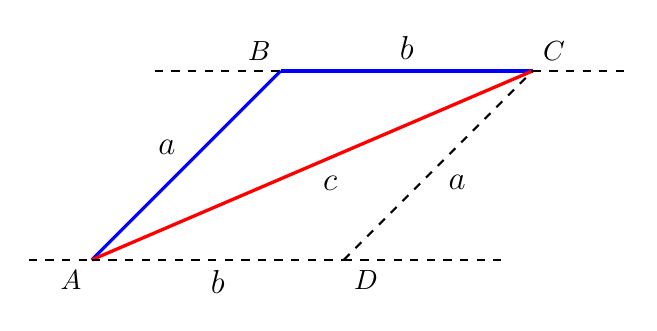
\begin{tikzpicture}[thick, scale = 0.8]
        \coordinate[label=below left:$A$] (A) at (0cm,0cm);
        \coordinate[label=above left:$B$] (B) at (3cm,3cm);
        \coordinate[label=above right:$C$] (C) at (7cm,3cm);
        \coordinate (D) at (-1cm,0cm);
        \coordinate (E) at (6.5cm,0cm);
        \coordinate (F) at (1cm,3cm);
        \coordinate (G) at (8.5cm,3cm);
        \coordinate[label=below right:$D$] (H) at (4cm,0cm);


        \draw [blue, very thick] (A) -- node[above left,black] {\large $a$} (B);
        \draw [blue, very thick] (B) -- node[above, black] {\large $b$} (C);
        \draw [red, very thick] (A) -- node[below right, black] {\large $c$} (C);
        \draw [dashed] (D) -- (A);
        \draw [dashed] (A) -- node[below, black] {\large $b$} (H);
        \draw [dashed] (H) -- (E);
        \draw [dashed] (F) -- (B);
        \draw [dashed] (C) -- (G);
        \draw [dashed] (H) -- node[below right, black] {\large $a$} (C);

        \tkzMarkAngle[arc=l, size=0.8cm, mark=none](E,A,B)
        \tkzLabelAngle[pos = 1.2](E,A,C){$\upalpha$}
    \end{tikzpicture}

    $c = \sqrt{a^2 + b^2 + 2 a b\cos\upalpha}$
\end{multicols}
\newpage
\begin{multicols}{2}
    \subsubsection{Stumpfer Winkel zwischen Vektoren}


    \begin{tikzpicture}[thick]
        \coordinate (A) at (0cm,0cm);
        \coordinate (B) at (-2cm,3cm);
        \coordinate (C) at (2cm,3cm);
        \coordinate (D) at (4cm,0cm);

        % angle
        \tkzMarkAngle[arc=l, size=0.8cm, mark=none](D,A,B)
        \tkzLabelAngle[pos = 1.2](D,A,B){$\upalpha$}

        \draw [blue, -Latex, very thick] (A) -- node[below left,black] {\large $\vv{a}$}(B);
        \draw [blue, -Latex, very thick] (A) -- node[below,black] {\large $\vv{b}$}(D);

    \end{tikzpicture}

    \begin{tikzpicture}[thick, scale = 0.9]
        \coordinate [label=below left:$A$](A) at (0cm,0cm);
        \coordinate [label=above left:$B$](B) at (-2cm,3cm);
        \coordinate [label=above right:$C$](C) at (2cm,3cm);
        \coordinate [label=below right:$D$](D) at (4cm,0cm);

        \draw [blue, -Latex, very thick] (A) -- node[below left,black] {\large $\vv{a}$}(B);
        \draw [dashed] (B) -- (C);
        \draw [red, -Latex, very thick] (A) -- (C);
        \draw [blue, -Latex, very thick] (A) -- node[below,black] {\large $\vv{b}$}(D);
        \draw [dashed] (D) -- (C);

        \draw (4.2cm,2.8cm) node {\large $\vv{c} =\vv{a}+\vv{b}$};
    \end{tikzpicture}\hspace{0.5cm}

    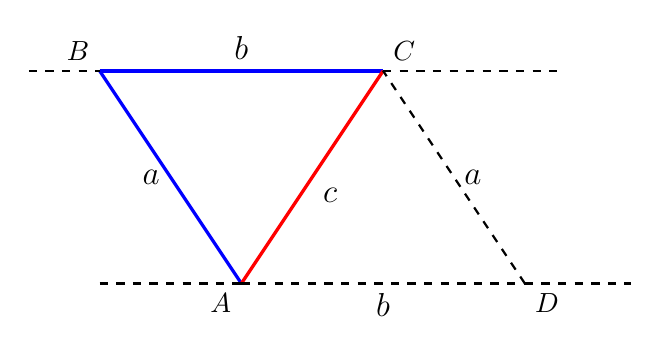
\begin{tikzpicture}[thick, scale = 0.9]
        \coordinate[label=below left:$A$] (A) at (0cm,0cm);
        \coordinate[label=above left:$B$] (B) at (-2cm,3cm);
        \coordinate[label=above right:$C$] (C) at (2cm,3cm);
        \coordinate (D) at (-2cm,0cm);
        \coordinate (E) at (5.5cm,0cm);
        \coordinate (F) at (-3cm,3cm);
        \coordinate (G) at (4.5cm,3cm);
        \coordinate[label=below right:$D$] (H) at (4cm,0cm);


        \tkzLabelAngle[pos = 0.7, right](A,B,C){\small $\upbeta$}

        \tkzLabelAngle[pos = 0.7, left](B,A,D){\small $\upbeta$}

        \draw [blue, very thick] (A) -- node[left,black] {\large $a$} (B);
        \draw [blue, very thick] (B) -- node[above, black] {\large $b$} (C);
        \draw [red, very thick] (A) -- node[below right, black] {\large $c$} (C);
        \draw [dashed] (D) -- (A);
        \draw [dashed] (A) -- node[below, black] {\large $b$} (H);
        \draw [dashed] (H) -- (E);
        \draw [dashed] (F) -- (B);
        \draw [dashed] (C) -- (G);
        \draw [dashed] (H) -- node[right, black] {\large $a$} (C);

        \tkzMarkAngle[arc=l, size=0.6cm, mark=none](E,A,B)
        \tkzLabelAngle[pos = 1](C,A,B){$\upalpha$}
    \end{tikzpicture}

    \[c = \sqrt{a^2 + b^2 + 2 a b\cos\upalpha}\]




    \subsection{Vektoren im Koordinatensystem}

    \subsubsection{Beziehungen zwischen Anfang und End Koordinaten}


    \begin{tikzpicture}[scale=0.6]
        \begin{axis}[
                axis lines=middle,
                axis line style = thick,
                axis equal image,
                grid=major,
                xmin=-2,
                xmax=9,
                ymin=-2,
                ymax=6,
                xlabel=$x$,
                ylabel=$y$,
                xlabel style={below right},
                ylabel style={left},
                xtick={-1,...,8},
                ytick={-1,...,5},
                yticklabels={,,},
                xticklabels={,,},
                %axis on top,
                %tick style={thick},
                width=12cm
            ]
        \end{axis}
        \coordinate (A) at (2.84cm,2.84cm);
        \coordinate (B) at (8.535cm,5.685cm);
        \coordinate [label=below:\large $x_1$](C) at (2.84cm,1.8cm);
        \coordinate [label=below:\large $x_2$](D) at (8.535cm,1.887cm);
        \coordinate [label=below:\large $0$](O) at (1.54cm,1.86cm);
        \coordinate (CC) at (2.84cm,1.2cm);
        \coordinate (DD) at (8.535cm,1.2cm);
        \coordinate [label=left:\large $y_1$](E) at (1.8cm,2.84cm);
        \coordinate [label=left:\large $y_2$](F) at (1.8cm,5.685cm);
        \coordinate (EE) at (1.1cm,2.84cm);
        \coordinate (FF) at (1.1cm,5.685cm);

        \draw [-Latex, ultra thick] (A) --  node[above left,black] {\large $\vv{a}$} (B);

        \draw[dashed, thick] (A) -- (C);
        \draw[dashed, thick] (A) -- (E);
        \draw[dashed, thick] (B) -- (D);
        \draw[dashed, thick] (B) -- (F);
        \draw [decorate, decoration={brace, mirror, amplitude=10pt}] (CC) -- (DD);
        \draw [left, decorate, decoration={brace, amplitude=10pt}] (EE) -- (FF);
        \draw (5.6cm,0.4cm) node {\large $a_x = x_2 - x_1$};
        \draw (-0.8cm,4.3cm) node {\large $a_y = y_2 - y_1$};
    \end{tikzpicture}
    \subsubsection{Der Vektor ist parallel oder senkrecht zur Koordinatenachse}

    \begin{tikzpicture}[scale=0.6]
        \begin{axis}[
                axis lines=middle,
                axis line style = thick,
                axis equal image,
                grid=major,
                xmin=-2,
                xmax=9,
                ymin=-2,
                ymax=6,
                xlabel=$x$,
                ylabel=$y$,
                xlabel style={below right},
                ylabel style={left},
                xtick={-1,...,8},
                ytick={-1,...,5},
                yticklabels={,,},
                xticklabels={,,},
                %tick style={thick},
                width=12cm
            ]
        \end{axis}
        % a
        \coordinate (A) at (2.84cm,2.84cm);
        \coordinate (B) at (6.63cm,2.84cm);
        \coordinate [label=below:$x_1$](C) at (2.84cm,1.8cm);
        \coordinate [label=below:$x_2$](D) at (6.63cm,1.8cm);
        \coordinate [label=below:\large $0$](O) at (1.54cm,1.86cm);
        \coordinate (CC) at (2.84cm,1.2cm);
        \coordinate (DD) at (6.63cm,1.2cm);
        \coordinate (E) at (1.8cm,2.84cm);
        % g
        \coordinate [label=left:$y_1$](CCC) at (1.8cm,6.63cm);
        \coordinate [label=left:$y_2$](DDD) at (1.8cm,3.78cm);
        \coordinate (FF) at (1.1cm,6.63cm);
        \coordinate (EE) at (1.1cm,3.78cm);
        \coordinate (F) at (8.535cm,1.88cm);
        \coordinate (FFF) at (8.535cm,6.63cm);
        \coordinate (EEE) at (8.535cm,3.78cm);
        %a
        \draw [-Latex, ultra thick] (A) --  node[above,black] {\large $\vv{a}$} (B);
        %g
        \draw [-Latex, ultra thick] (FFF) --  node[right,black] {\large $\vv{g}$} (EEE);

        \draw[dashed, thick] (A) -- (C);
        \draw[dashed, thick] (E) -- (A);
        \draw[dashed, thick] (CCC) -- (FFF);
        \draw[dashed, thick] (DDD) -- (EEE);

        % right angle
        \draw (1.9,2.55)-|(2.2,2.85);
        \draw (8.235,1.89)|-(8.535,2.19);

        \draw[dashed, thick] (B) -- (D);
        \draw[dashed, thick] (EEE) -- (F);
        \draw [decorate, decoration={brace, mirror, amplitude=10pt}] (CC) -- (DD);
        \draw [left, decorate, decoration={brace, amplitude=10pt}] (EE) -- (FF);
        \draw (5cm,0.5cm) node {$\hly{a_x=x_2 - x_1 = a}$};
        \draw (1cm,2.8cm) node {$\hly{a_y=0}$};
        \draw (8.55cm,1.4cm) node {$\hlt{g_x=0}$};
        \draw (-1.2cm,5.2cm) node {$\hlt{g_y=y_2-y_1 = -g}$};
    \end{tikzpicture}
    \subsubsection{Der Vektor ist in einem beliebigen Winkel zur Koordinatenachse gerichtet
    }
    \begin{tikzpicture}[scale=0.7]
        \begin{axis}[
                axis lines=middle,
                axis line style = thick,
                axis equal image,
                grid=major,
                xmin=-2,
                xmax=9,
                ymin=-2,
                ymax=6,
                xlabel=$x$,
                ylabel=$y$,
                xlabel style={below right},
                ylabel style={left},
                xtick={-1,...,8},
                ytick={-1,...,5},
                yticklabels={,,},
                xticklabels={,,},
                %tick style={thick},
                width=12cm
            ]
        \end{axis}
        \coordinate [label=above left:\large $A$](A) at (2.84cm,2.84cm);
        \coordinate [label=above right:\large $C$](B) at (8.535cm,5.685cm);
        \coordinate [label=below:\large $x_1$](C) at (2.84cm,1.8cm);
        \coordinate [label=below:\large $x_2$](D) at (8.535cm,1.887cm);
        \coordinate [label=below:\large $0$](O) at (1.54cm,1.86cm);
        \coordinate (CC) at (2.84cm,1.2cm);
        \coordinate (DD) at (8.535cm,1.2cm);
        \coordinate [label=left:\large $y_1$](E) at (1.8cm,2.84cm);
        \coordinate [label=left:\large $y_2$](F) at (1.8cm,5.685cm);
        \coordinate (EE) at (1.1cm,2.84cm);
        \coordinate (FF) at (1.1cm,5.685cm);
        \coordinate [label=above right:\large $B$](GG) at (8.535cm,2.84cm);

        \draw [-Latex, ultra thick] (A) --  node[above left,black] {\large $\vv{a}$} (B);

        \draw[dashed, thick] (A) -- (C);
        \draw[dashed, thick] (E) -- (GG);
        % right angle
        \draw (8.235,2.84)|-(8.535,3.14);
        % angle
        \tkzMarkAngle[arc=l, size=1cm, mark=none](GG,A,B)
        \tkzLabelAngle[pos = 1.4](GG,A,B){$\upalpha$}
        \draw[dashed, thick] (B) -- (D);
        \draw[dashed, thick] (B) -- (F);
        \draw [decorate, decoration={brace, mirror, amplitude=10pt}] (CC) -- (DD);
        \draw [left, decorate, decoration={brace, amplitude=10pt}] (EE) -- (FF);
        \draw (5.4cm,2.4cm) node {\large $\hly{a_x = a\cos{\upalpha}}$};
        \draw (10.1cm,4.1cm) node {\large $\hly{a_y = a\sin{\upalpha}}$};
        \draw (5.6cm,0.5cm) node {\large $a_x>0$};
        \draw (0cm,4.2cm) node {\large $a_y>0$};
    \end{tikzpicture}

    \begin{tikzpicture}[scale=0.7]
        \begin{axis}[
                axis lines=middle,
                axis line style = thick,
                axis equal image,
                grid=major,
                xmin=-2,
                xmax=9,
                ymin=-2,
                ymax=6,
                xlabel=$x$,
                ylabel=$y$,
                xlabel style={below right},
                ylabel style={left},
                xtick={-1,...,8},
                ytick={-1,...,5},
                yticklabels={,,},
                xticklabels={,,},
                %tick style={thick},
                width=12cm
            ]
        \end{axis}
        \coordinate [label=above left:\large $A$](A) at (2.84cm,2.84cm);
        \coordinate [label=above right:\large $C$](B) at (8.535cm,5.685cm);
        \coordinate [label=below:\large $x_2$](C) at (2.84cm,1.8cm);
        \coordinate [label=below:\large $x_1$](D) at (8.535cm,1.887cm);
        \coordinate [label=below:\large $0$](O) at (1.54cm,1.86cm);
        \coordinate (CC) at (2.84cm,1.2cm);
        \coordinate (DD) at (8.535cm,1.2cm);
        \coordinate [label=left:\large $y_2$](E) at (1.8cm,2.84cm);
        \coordinate [label=left:\large $y_1$](F) at (1.8cm,5.685cm);
        \coordinate (EE) at (1.1cm,2.84cm);
        \coordinate (FF) at (1.1cm,5.685cm);
        \coordinate [label=above right:\large $B$](GG) at (8.535cm,2.84cm);

        \draw [-Latex, ultra thick] (B) --  node[above left,black] {\large $\vv{a}$} (A);

        \draw[dashed, thick] (A) -- (C);
        \draw[dashed, thick] (E) -- (GG);
        % right angle
        \draw (8.235,2.84)|-(8.535,3.14);
        % angle
        \tkzMarkAngle[arc=l, size=1cm, mark=none](GG,A,B)
        \tkzLabelAngle[pos = 1.4](GG,A,B){$\upalpha$}
        \draw[dashed, thick] (B) -- (D);
        \draw[dashed, thick] (B) -- (F);
        \draw [decorate, decoration={brace, mirror, amplitude=10pt}] (CC) -- (DD);
        \draw [left, decorate, decoration={brace, amplitude=10pt}] (EE) -- (FF);
        \draw (5.4cm,2.4cm) node {\large $\hly{a_x = -a\cos{\upalpha}}$};
        \draw (10.2cm,4.1cm) node {\large $\hly{a_y = -a\sin{\upalpha}}$};
        \draw (5.6cm,0.5cm) node {\large $a_x<0$};
        \draw (0cm,4.2cm) node {\large $a_y<0$};
    \end{tikzpicture}

    \begin{tikzpicture}[scale=0.7]
        \begin{axis}[
                axis lines=middle,
                axis line style = thick,
                axis equal image,
                grid=major,
                xmin=-2,
                xmax=9,
                ymin=-2,
                ymax=6,
                xlabel=$x$,
                ylabel=$y$,
                xlabel style={below right},
                ylabel style={left},
                xtick={-1,...,8},
                ytick={-1,...,5},
                yticklabels={,,},
                xticklabels={,,},
                %tick style={thick},
                width=12cm
            ]
        \end{axis}
        \coordinate (A) at (2.84cm,2.84cm);
        \coordinate (B) at (8.535cm,5.685cm);
        \coordinate [label=below:\large $x_2$](C) at (2.84cm,1.8cm);
        \coordinate [label=below:\large $x_1$](D) at (8.535cm,1.887cm);
        \coordinate [label=below:\large $0$](O) at (1.54cm,1.86cm);
        \coordinate (CC) at (2.84cm,1.2cm);
        \coordinate (DD) at (8.535cm,1.2cm);
        \coordinate [label=left:\large $y_1$](E) at (1.8cm,2.84cm);
        \coordinate [label=left:\large $y_2$](F) at (1.8cm,5.685cm);
        \coordinate (EE) at (1.1cm,2.84cm);
        \coordinate (FF) at (1.1cm,5.685cm);
        \coordinate (GG) at (8.535cm,2.84cm);
        \coordinate (H) at (2.84cm,5.685cm);

        \draw [-Latex, ultra thick] (GG) --  node[above right,black] {\large $\vv{a}$} (H);

        \draw[dashed, thick] (H) -- (C);
        \draw[dashed, thick] (E) -- (GG);
        %\draw[dashed, thick] (E) -- (GG);
        % right angle
        \draw (2.84,3.14)-|(3.14,2.84);
        \draw (8.235,5.685)|-(8.535,5.385);
        % angle
        \tkzMarkAngle[arc=l, size=0.8cm, mark=none](B,GG,H)
        \tkzLabelAngle[pos = 1.2](B,GG,H){$\upalpha$}
        \tkzMarkAngle[arc=l, size=0.8cm, mark=none](A,H,GG)
        \tkzLabelAngle[pos = 1.2](A,H,GG){$\upalpha$}
        \draw[dashed, thick] (B) -- (D);
        \draw[dashed, thick] (B) -- (F);
        \draw [decorate, decoration={brace, mirror, amplitude=10pt}] (CC) -- (DD);
        \draw [left, decorate, decoration={brace, amplitude=10pt}] (EE) -- (FF);
        \draw (5.4cm,2.4cm) node {\large $\hly{a_x = -a\sin{\upalpha}}$};
        \draw (10.2cm,4.1cm) node {\large $\hly{a_y = a\cos{\upalpha}}$};
        \draw (5.6cm,0.5cm) node {\large $a_x<0$};
        \draw (0cm,4.2cm) node {\large $a_y>0$};
    \end{tikzpicture}


    \newpage
\end{multicols}
\begin{multicols}{2}


    \subsection{Diverses}
    \subsubsection{Lineare Abhängigkeit zweier Vektoren}
    Zwei Vektoren heißen linear abhängig, wenn es zwei Zahlen $\lambda_1$ und $\lambda_2$ gibt, die nicht beide Null sind, so dass gilt:
    $\lambda_1\vec{a_1} + \lambda_2\vec{a_2} = \vec{0}$

    \textbf{Verfahren 1}

    Zwei Vektoren des $\mathbb{R}^2$ sind genau dann linear abhängig, wenn sie Vielfache voneinander sind.

    \textbf{Verfahren 2}

    Zwei Vektoren des $\mathbb{R}^2$ sind genau dann linear abhängig, wenn ihre Determinante gleich Null ist.

    $\text{Determinate} = \begin{vmatrix} {\color{red}a} & {\color{blue}b} \\ {\color{blue}c} & {\color{red}d} \end{vmatrix} = {\color{red}a}\cdot{\color{red}d}-{\color{blue}c}\cdot{\color{blue}b}$

    \textbf{Eigenschaften}

    Zwei Vektoren des $\mathbb{R}^2$ sind genau dann linear abhängig, wenn sie parallel sind.\\
    Mehr als zwei Vektoren des $\mathbb{R}^2$ sind stets linear abhängig.

    Begründung: Der $\mathbb{R}^2$ ist definiert als ein Vektorraum, der durch zwei linear unabhängige, also nicht parallele Vektoren aufgespannt wird. Diese zwei Vektoren nennt man Basis des Vektorraums. Meist verwendet man die sog. Standardbasis (kanonische Basis):
    \subsubsection{Lineare Abhängigkeit dreier Vektoren}

    Drei Vektoren heißen linear abhängig, wenn es drei Zahlen $\lambda_1$  $\lambda_2$ und $\lambda_3$ gibt, die nicht alle gleich Null sind, so dass gilt:
    $\lambda_1\vec{a_1} + \lambda_2\vec{a_2} + \lambda_3\vec{a_3} = \vec{0}$

    Oder: Drei Vektoren sind genau dann linear abhängig, wenn sich der Nullvektor durch eine Linearkombination der Vektoren erzeugen lässt.

    \textbf{Verfahren 1}

    Drei Vektoren des $\mathbb{R}^3$ sind genau dann linear abhängig, wenn die Anwendung des Gauß-Algorithmus zu einer Nullzeile führt.

    \textbf{Verfahren 2}
    Drei Vektoren des $\mathbb{R}^3$ sind genau dann linear abhängig, wenn ihre Determinante gleich Null ist.

    \begin{align*} \text{Determinante}= \begin{vmatrix} a & b & c \\ d & e & f \\ g & h & i \end{vmatrix}=\end{align*}
    $a \cdot e \cdot i + b \cdot f \cdot g + c \cdot d \cdot h - g \cdot e \cdot c - h \cdot f \cdot a - i \cdot d \cdot b$

    \textbf{Eigenschaften}

    Zwei Vektoren des $\mathbb{R}^3$ sind genau dann linear abhängig, wenn sie parallel sind.

    Drei Vektoren des $\mathbb{R}^3$ sind genau dann linear abhängig, wenn sie in einer Ebene liegen – dort können sie untereinander auch parallel sein.

    Mehr als drei Vektoren des $\mathbb{R}^3$ sind stets linear abhängig.

    \subsection{Punkt Gerade Ebene Berechnungen}
    \subsubsection{Liegt Punkt auf Gerade oder Ebene?}
    Generell muss man bei diesem Problem folgendes haben: Einen Punkt (X;Y;Z), eine Gerade in Hessesche Normalform und eine Ebene
    (Koordinatform oder Hessesche Normalform).

    Um zu testen ob der Punkt auf der Geraden liegt setzt man den Punkt in die Hessesche Normalforn $\begin{pmatrix} X \\ Y \\ Z \end{pmatrix}$ und erstellt dann
    3 Gleichungen um die Variable der Gerade zu erhalten.

    Setze die Variable von einer dieser Gleichung in die anderen 2 Gleichungen ein um zu testen ob es funktioniert.

    Um zu testen ob der Punkt auf der Ebene liegt kann man den Punkt in die koordinaten Ebene einsetzen und gleich Null stellen.
    \section{Gut Glück Kätzchen}
    Für Emotionale Unterstützung während der Prüfung.


    \begin{center}
        \includegraphics[scale=0.7]{veryimportant.png}
    \end{center}


    \newpage
\end{multicols}